
% This LaTeX was auto-generated from MATLAB code.
% To make changes, update the MATLAB code and republish this document.

\documentclass{article}
\usepackage{graphicx}
\usepackage{color}

\sloppy
\definecolor{lightgray}{gray}{0.5}
\setlength{\parindent}{0pt}

\begin{document}

    
    
\section*{Spaceflight Mechanics - Semester Project - Spring 2019}

\begin{par}
Angles Only Orbit Determination of Unknown Object from a Known Satellite
\end{par} \vspace{1em}

\subsection*{Contents}

\begin{itemize}
\setlength{\itemsep}{-1ex}
   \item Administrative Remarks
   \item Clearing figures and command line
   \item Declaring constants
   \item Measured angle values
   \item Time vectors
   \item Calculate position R at the three times of the known satellite from known satellite orbital parameters
   \item Determining unit vectors from satellite to unknown object
   \item Cross products among the direction cosine vectors
   \item Computing the six scalar quantities
   \item Calculating A and B
   \item Calculating E
   \item Calculating a, b, and c
   \item Calculating the roots numerically
   \item Calculating the Lagrange coefficients
   \item Calculating position vector magnitudes from satellite to unknown object
   \item Calculating position vectors from earth center to unknown object
   \item Calculating velocity of unknown object
   \item Method to improve accuracy of results taken from Curtis
   \item Determing orbit elements of unknown object from r2 and v2
   \item Plotting both orbits of known satellite and unknown object
   \item Ouputting parameters to Command Line
\end{itemize}


\subsection*{Administrative Remarks}

\begin{verbatim}
%Author: Johnathan Corbin
%February 9, 2019
%--------------------------------------------------------------------------
%Assumptions made about the system:
% - The two body problem applies.
% - This system takes place around the Earth (u = 398600).
% - The Earth is a perfect sphere so as to ignore effects of precession.
% - I use the topocentric horizon reference frame on the spacecraft to
%    create the direction unit vectors to the unknown object from a given
%    altitude and azimuth angle seen from the spacecraft.
% - The timescale between angle measurements must be fairly small so that
%    only the first terms of the Lagrange coefficients are large enough to
%    significantly contribute.
% - The orbit of the satellite taking the measurements is known and that a
%      position vector can be made to that satellite at each instance when
%      an angle measurement is made.
% - Values of the estimated orbit are output at the end of the script, any
%      value that is a rotation value are in degrees, not radians.
%--------------------------------------------------------------------------
% Derivations of the algorithm and some of the required functions were
% pulled from Orbital Mechanics for Engineering Students by Howard D.
% Curtis.
%--------------------------------------------------------------------------
%Required functions:
% f_and_g, kepler_E, kepler_U, orbit_elements, satellite, posroot, stumpC,
% stumpS
%--------------------------------------------------------------------------
\end{verbatim}


\subsection*{Clearing figures and command line}

\begin{verbatim}
clear, clc
close all
\end{verbatim}


\subsection*{Declaring constants}

\begin{verbatim}
global u

u = 398600; %gravitational parameter for earth
r_earth = 6378; %radius of earth
deg_rad = pi / 180; %converting degree to rad
\end{verbatim}


\subsection*{Measured angle values}

\begin{verbatim}
azimuth = [10, 89,  90] * deg_rad; %Azimuth angle of unknown object at times
%10 20 30 to generate hyperbolic
altitude = [0, 20, 40] * deg_rad; %Altitude angle of unkown object at times
\end{verbatim}


\subsection*{Time vectors}

\begin{verbatim}
t = [0, 5*60, 10*60]; %Array for time values, seconds
tau = [t(1) - t(2), 0, t(3) - t(2)]; %Calculating time intervals
T = tau(3) - tau(1);
\end{verbatim}


\subsection*{Calculate position R at the three times of the known satellite from known satellite orbital parameters}

\begin{verbatim}
e_sat = 0;
a_sat = 8000;
Omega_sat = 0;
i_sat = 0;
omega_sat = 0;
anomaly = pi / 4;

[sat_orbit, R] = satellite(e_sat, a_sat, Omega_sat, omega_sat, i_sat, anomaly, t);

%R = [5582.84, 0, 3073.9;...
 %   5581.5, 122.122, 3073.9;...
  %  5577.7, 244.186, 3073.9];
%Random position vectors to test algorithm
\end{verbatim}


\subsection*{Determining unit vectors from satellite to unknown object}

\begin{verbatim}
p = zeros(3); %Creating array for direction cosine vectors at the three times

%For loop to calculate the direction cosine vectors at each time
for i = 1:3
    p(i,1) = cos(altitude(i)) * sin(azimuth(i));
    p(i,2) = cos(altitude(i)) * cos(azimuth(i));
    p(i,3) = sin(altitude(i));
end

%p = [.846428, 0, .532504;...
 %   .74929, .463023, .47347;...
  %  .529447, .777163, .340152];
% Random direction cosine vectors to test algorithm
\end{verbatim}


\subsection*{Cross products among the direction cosine vectors}

\begin{verbatim}
p1 = cross(p(2,:),p(3,:));
p2 = cross(p(1,:),p(3,:));
p3 = cross(p(1,:),p(2,:));

D0 = dot(p(1,:),p1);
\end{verbatim}


\subsection*{Computing the six scalar quantities}

\begin{verbatim}
D = zeros(3);
for q = 1:3
   D(q,1) = dot(R(q,:), p1);
   D(q,2) = dot(R(q,:), p2);
   D(q,3) = dot(R(q,:), p3);
end
\end{verbatim}


\subsection*{Calculating A and B}

\begin{verbatim}
A = (-D(1,2)*tau(3)/T + D(2,2) + D(3,2) * tau(1) / T) / D0;
B = (D(1,2)*(tau(3)^2 - T^2)*tau(3)/T + D(3,2)*(T^2 - tau(1)^2) * tau(1)/T)/(6 * D0);
\end{verbatim}


\subsection*{Calculating E}

\begin{verbatim}
E = dot(R(2,:), p(2,:));
\end{verbatim}


\subsection*{Calculating a, b, and c}

\begin{verbatim}
a = -(A^2 + 2*A*E + (norm(R(2,:)))^2);
b = -2*u*B*(A + E);
c = -(u^2 * B^2);
\end{verbatim}


\subsection*{Calculating the roots numerically}

\begin{verbatim}
Roots = roots([1 0 a 0 0 b 0 0 c]);
x = posroot(Roots);
\end{verbatim}


\subsection*{Calculating the Lagrange coefficients}

\begin{verbatim}
f1 = 1 - (u*tau(1)^2/x^3)/2;
f3 = 1 - (u*tau(3)^2/x^3)/2;

g1 = tau(1) - (u*(tau(1)/x)^3)/6;
g3 = tau(3) - (u*(tau(3)/x)^3)/6;
\end{verbatim}


\subsection*{Calculating position vector magnitudes from satellite to unknown object}

\begin{verbatim}
P1 = 1/D0*((6*(D(3,1)*tau(1)/tau(3) + D(2,1)*T/tau(3))*x^3 + u*D(3,1)*(T^2 - tau(1)^2)*tau(1)/tau(3))/(6*x^3 + u*(T^2 - tau(3)^2)) - D(1,1));
P2 = A + u * B / x^3;
P3 = 1/D0*((6*(D(1,3)*tau(3)/tau(1) - D(2,3)*T/tau(1))*x^3 + u*D(1,3)*(T^2 - tau(3)^2)*tau(3)/tau(1))/(6*x^3 + u*(T^2 - tau(1)^2)) - D(3,3));
\end{verbatim}


\subsection*{Calculating position vectors from earth center to unknown object}

\begin{verbatim}
r1 = R(1,:) + P1*p(1,:);
r2 = R(2,:) + P2*p(2,:);
r3 = R(3,:) + P3*p(3,:);
\end{verbatim}


\subsection*{Calculating velocity of unknown object}

\begin{verbatim}
v2 = (1 / (f1*g3 - f3*g1))*(-f3*r1 + f1*r3);
\end{verbatim}


\subsection*{Method to improve accuracy of results taken from Curtis}

\begin{verbatim}
P1_old = P1;  P2_old = P2;  P3_old = P3;
diff1    = 1;     diff2    = 1;     diff3    = 1;
n    = 0;
nmax = 2000;
tol  = 1.e-10;

%...Iterative improvement loop from Curtis:
while ((diff1 > tol) && (diff2 > tol) && (diff3 > tol)) && (n < nmax)
    n = n+1;

%...Compute quantities required by universal kepler's equation:
    ro  = norm(r2);
    vo  = norm(v2);
    vro = dot(v2,r2)/ro;
    alpha   = 2/ro - vo^2/u;

%...Solve universal Kepler's equation at times tau1 and tau3 for
%   universal anomalies x1 and x3:
    x1 = kepler_U(tau(1), ro, vro, alpha);
    x3 = kepler_U(tau(3), ro, vro, alpha);

%...Calculate the Lagrange f and g coefficients at times tau1
%   and tau3:
    [ff1, gg1] = f_and_g(x1, tau(1), ro, alpha);
    [ff3, gg3] = f_and_g(x3, tau(3), ro, alpha);

%...Update the f and g functions at times tau1 and tau3 by
%   averaging old and new:
    f1    = (f1 + ff1)/2;
    f3    = (f3 + ff3)/2;
    g1    = (g1 + gg1)/2;
    g3    = (g3 + gg3)/2;

%...Equations 5.96 and 5.97:
    c1    =  g3/(f1*g3 - f3*g1);
    c3    = -g1/(f1*g3 - f3*g1);

%...Equations 5.109a, 5.110a and 5.111a:
    P1  = 1/D0*(      -D(1,1) + 1/c1*D(2,1) - c3/c1*D(3,1));
    P2  = 1/D0*(   -c1*D(1,2) +      D(2,2) -    c3*D(3,2));
    P3  = 1/D0*(-c1/c3*D(1,3) + 1/c3*D(2,3) -       D(3,3));

%...Equations 5.86:
    r1 = R(1,:) + P1*p(1,:);
    r2 = R(2,:) + P2*p(2,:);
    r3 = R(3,:) + P3*p(3,:);

%...Equation 5.118:
    v2    = (-f3*r1 + f1*r3)/(f1*g3 - f3*g1);

%...Calculate differences upon which to base convergence:
    diff1 = abs(P1 - P1_old);
    diff2 = abs(P2 - P2_old);
    diff3 = abs(P3 - P3_old);

%...Update the slant ranges:
    P1_old = P1;  P2_old = P2;  P3_old = P3;
end
%...End iterative improvement loop
\end{verbatim}


\subsection*{Determing orbit elements of unknown object from r2 and v2}

\begin{verbatim}
[mag_e, a, theta, Omega, inc, omega] = orbit_elements(r2, v2);
\end{verbatim}


\subsection*{Plotting both orbits of known satellite and unknown object}

\begin{verbatim}
    if (mag_e > 1)
        l_limit = -pi / 2;
        u_limit = pi / 2;
    else
        l_limit = 0;
        u_limit = 2 * pi;
    end

    %Converting estimated orbital parameters to radians
    W = Omega * deg_rad;
    w = omega * deg_rad;
    inclination = inc * deg_rad;

    %Computing direction cosine matrix from perifocal to N for unknown object
    C_N_PF_obj = [-sin(W)*cos(inclination)*sin(w)+cos(W)*cos(w), -sin(W)*cos(inclination)*cos(w)-cos(W)*sin(w), sin(W)*sin(inclination);...
        cos(W)*cos(inclination)*sin(w)+sin(W)*cos(w), cos(W)*cos(inclination)*cos(w) - sin(W)*sin(w), sin(inclination)*cos(w);...
        sin(inclination)*sin(w), sin(inclination)*cos(w), cos(inclination)];

    %Magnitude of momentum for unknown object
    h = norm(cross(r2, v2));

    %For loop to calculate X,Y,Z positions of the estimated orbit
    counter = 1;
    for angle = l_limit:.001:u_limit
        radius_polar = [h^2/(u * (1 + mag_e * cos(angle)));0;0];
        C_PF_polar_obj = [cos(angle), sin(angle), 0;...
        -sin(angle), cos(angle), 0;...
        0, 0, 1].';
       radius_pf = (C_PF_polar_obj * radius_polar);
       radius = (C_N_PF_obj * radius_pf).';
       for z = 1:3
           coordinate(z, counter) = radius(z);
       end
       counter = counter + 1;
    end
    per = 0;

    radius_polar = [h^2/(u * (1 + mag_e * cos(per)));0;0];
        C_PF_polar_obj = [cos(per), sin(per), 0;...
        -sin(per), cos(per), 0;...
        0, 0, 1].';
    radius_pf = (C_PF_polar_obj * radius_polar);
    radius = (C_N_PF_obj * radius_pf).';
    perogee = radius;

    %Plot the previously determined orbit
    plot3(coordinate(1,:), coordinate(2,:), coordinate(3,:), 'r')
    hold on

    %Plot the known orbit
    plot3(sat_orbit(1,:), sat_orbit(2,:), sat_orbit(3,:), 'b')

    %Plot a sphere to represent the Earth
    [xx, yy, zz] = sphere(100);
    lightGrey = 0.8*[1 1 1];
    surface(r_earth*xx, r_earth*yy, r_earth*zz, 'FaceColor', 'none', 'EdgeColor', lightGrey);

    %Draw and label the axes
    line([0 3*r_earth],   [0 0],   [0 0]); text(3*r_earth+1000,   0,   0, 'n_1')
    line(  [0 0], [0 3*r_earth],   [0 0]); text(  0, 3*r_earth+1000,   0, 'n_2')
    line(  [0 0],   [0 0], [0 3*r_earth]); text(  0,   0, 3*r_earth+1000, 'n_3')

    %Draw line to perogee
    line([0 perogee(1)], [0 perogee(2)], [0 perogee(3)], 'Color', 'k');
    text(perogee(1)*1.2, perogee(2)*1.2, perogee(3)*1.2, 'Perogee')

    %Draw line to each vector R of the known satellite at times
    line([0 R(1,1)], [0 R(1,2)], [0 R(1, 3)], 'Color', 'k', 'Linestyle', '-.')
    line([0 R(2,1)], [0 R(2,2)], [0 R(2, 3)], 'Color', 'k', 'Linestyle', '-.')
    line([0 R(3,1)], [0 R(3,2)], [0 R(3, 3)], 'Color', 'k', 'Linestyle', '-.')

    %Miscellanious graph adjustments
    grid on
    axis equal
    xlabel('km')
    ylabel('km')
    zlabel('km')
    view(3)
    title('Estimated Orbit Around Earth')
    legend('Estimated Orbit', 'Known Orbit')

    if (mag_e > -1) && (mag_e < 1)
        orbit = 'elliptical';
    else
        orbit = 'hyperbolic';
    end
\end{verbatim}

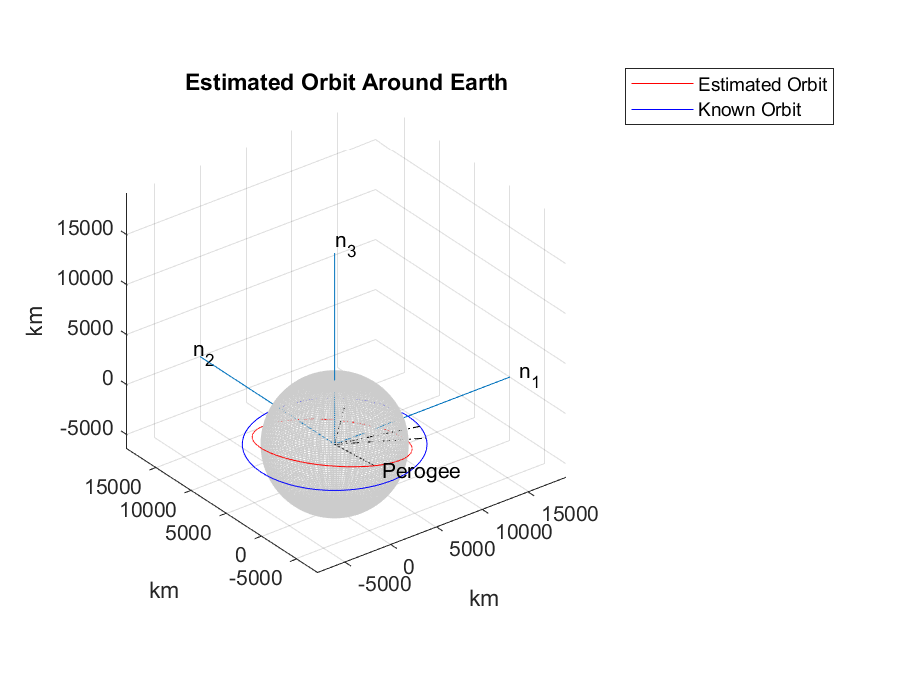
\includegraphics [width=4in]{Project_01.eps}


\subsection*{Ouputting parameters to Command Line}

\begin{verbatim}
fprintf('Estimated Orbital Parameters of the Unknown Object\n')
fprintf('------------------------------------------------------------------')
fprintf('\n Radius at point 2 [km] =                        %g n_1', r2(1))
fprintf('\n                                                 %g n_2', r2(2))
fprintf('\n                                                 %g n_3\n', r2(3))
fprintf('\n Velocity at point 2 [km/s] =                    %g n_1', v2(1))
fprintf('\n                                                 %g n_2', v2(2))
fprintf('\n                                                 %g n_3\n', v2(3))
fprintf('------------------------------------------------------------------')
fprintf('\n Orbit is %s.', orbit)
fprintf('\n Eccentricity =                                       %g', mag_e)
fprintf('\n Semi-Major Axis [km] =                              %g', a)
fprintf('\n Right of Ascension of the Ascending Node [degrees] = %g', Omega)
fprintf('\n Inclination [degrees] =                              %g', inc)
fprintf('\n Argument of Perogee [degrees] =                      %g', omega)
fprintf('\n True Anomaly [degrees] =                             %g', theta)
fprintf('\n')
fprintf('------------------------------------------------------------------')
fprintf('\n Closest approach to Earth [km] =                     %g', norm(perogee) - r_earth);
fprintf('\n')
\end{verbatim}

        \color{lightgray} \begin{verbatim}Estimated Orbital Parameters of the Unknown Object
------------------------------------------------------------------
 Radius at point 2 [km] =                        5391.05 n_1
                                                 -4006.92 n_2
                                                 -563.775 n_3

 Velocity at point 2 [km/s] =                    4.7191 n_1
                                                 5.95546 n_2
                                                 -1.80436 n_3
------------------------------------------------------------------
 Orbit is elliptical.
 Eccentricity =                                       0.0584521
 Semi-Major Axis [km] =                              6959.53
 Right of Ascension of the Ascending Node [degrees] = 123.722
 Inclination [degrees] =                              14.0104
 Argument of Perogee [degrees] =                      139.888
 True Anomaly [degrees] =                             60.3224
------------------------------------------------------------------
 Closest approach to Earth [km] =                     174.733
\end{verbatim} \color{black}
    


\end{document}
    
